%----------------------------------------------------------------------------
\chapter{Irodalomkutatás}
%----------------------------------------------------------------------------

A legjelentősebb katonai hatalmak mindegyike rendelkezik távvezérelt fegyverrendszerekkel, leggyakrabban valamilyen távolról irányított gépfegyver formájában. Azonban se az egyes országok nemzetbiztonságának, se a fegyveripari partnercégeknek nem áll érdekében a szükségesnél több információt kiadni. Ez egy kicsit megnehezítette az irodalomkutatást, de a képek alapján azért sok információt ki lehet nyerni.

\section{Megvalósult rendszerek} \label{sec:valos}

\paragraph{CROWS \cite{crows}}
Az egyik legnagyobb darabszámban gyártott távirányított fegyverrendszer az amerikai \textsl{CROWS} rendszer, amely a NATO-országokban, köztük Magyarországon is rendszeresített. Ennek értelmében telepíthető sok NATO által használt páncélozott járműre, köztük a Humvee-ra, a Stryker-re, és a Buffalo MRAP-re. Több verziója létezik több kaliberrel, a \ref{fig:irod_crows}. ábrán egy M240B géppuskával látható.\\

\begin{figure}[h!]
	\centering
	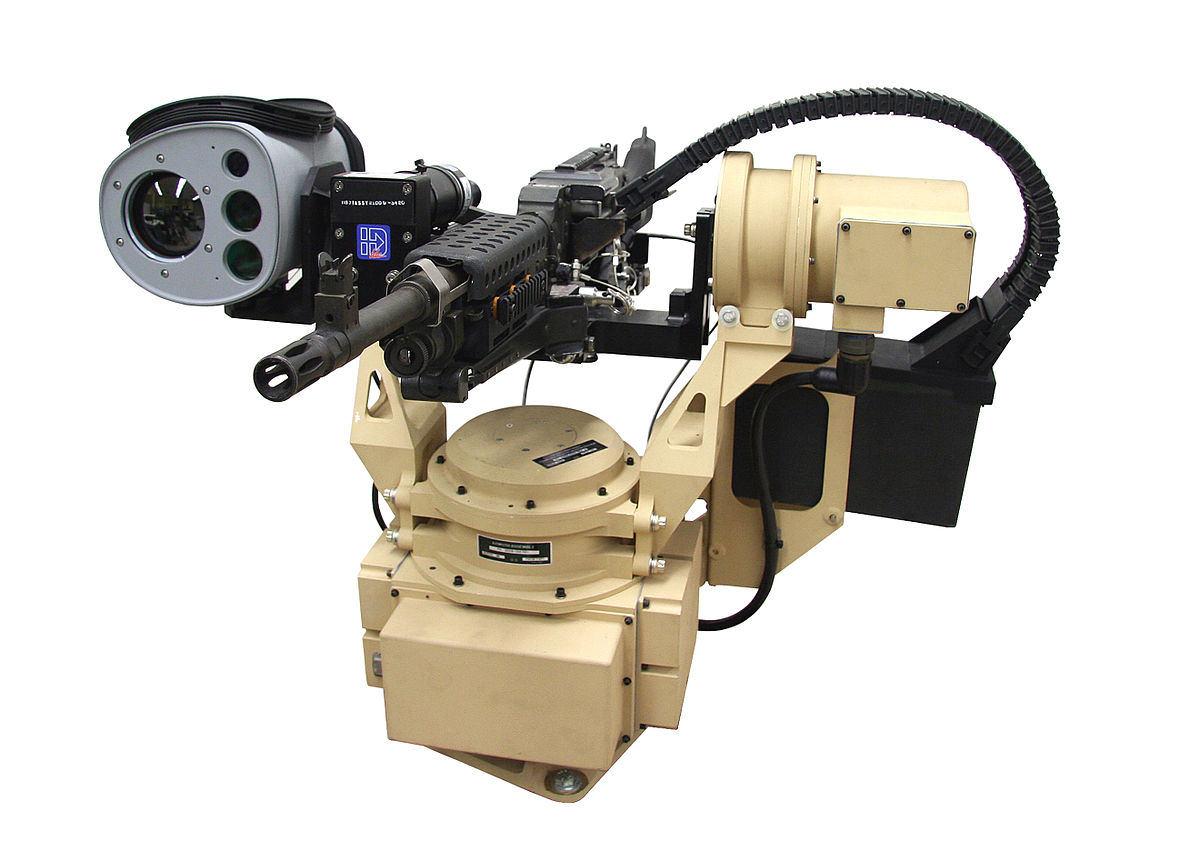
\includegraphics[width=.6\linewidth]{irod_crows}
	\caption{Az amerikai CROWS rendszer \cite{crows}}
	\label{fig:irod_crows}
\end{figure}

A szerelék a fegyverrel együtt $360^\circ$-ban képes elfordulni, és $-20^{\circ}$-tól $+60^{\circ}$-ig tud billenni. A fegyvercső giroszkóppal stabilizált. A kezelő egy 15 hüvelykes kijelzőn tud célozni a fegyverrel. A rendszer a sima kamera mellett rendelkezik hőkamerával is, így éjszaka is használható. Mind a két kamera el van látva lézeres távolságmérővel, amivel rá lehet állni a célpontra, és a jármű mozgása közben is lehet azt követni. A kamerát és a fegyvert lehet külön is mozgatni, ami azért hasznos, mert anélkül lehet követni a gyanús alakok mozgását, hogy félelmet keltenénk az emberekben.

\paragraph{Arbalet-DM \cite{arbalet}}
A \textsl{CROWS} rendszer orosz megfelelője a hasonló kialakítású \textsl{Arbalet-DM} (\ref{fig:irod_arbalet}.ábra). Ennek a rendszernek az alapja a 12.7 mm-es KORD nehézgéppuska. Rendelkezik 4 gránátvetővel is, amelyek füstfüggöny felhúzására használható. A kamera és a fegyver elhelyezése, de még a lőszer pozíciója is teljesen hasonló az amerikai párjához.

\begin{figure}[h!]
	\centering
	\includegraphics[width=.5\linewidth]{irod_arbalet}
	\caption{Az orosz Arbalet-DM rendszer \cite{arbalet}}
	\label{fig:irod_arbalet}
\end{figure}

A rendszer $360^\circ$-ban képes elfordulni, és $-20^{\circ}$-tól $+70^{\circ}$-ig tud billenni, tehát egy kicsit nagyobb részt tud lefedni, mint a CROWS. A hatótáv nappal 2000 m, éjszaka 1500 m. Ez a rendszer is el van látva hőkamerával és lézeres távolságmérővel.

\paragraph{DeFNder \cite{defnder}}
A következő megoldás a belga \textsl{DeFNder} termékcsalád, amelynek két tagja a \textsl{Light} és a \textsl{Medium}(\ref{fig:irod_defnder}. ábra). Értelem szerűen kettő közül az utóbbi az, amelyre nehezebb fegyverzetet lehet telepíteni. A függőleges tengelyen $360^\circ$-ban képes elfordulni 90 fok/másodperc sebességgel, a vízszintes tengelyen $-45^{\circ}$-tól $+75^{\circ}$-ig tud billenni, 60 fok/másodperc sebességgel. Opcionálisan ellátható infravörös- és hőkamerával a rossz látási körülmények esetére, valamint lézeres távolságmérővel a ballisztikai kompenzációhoz.
\begin{figure}[h!]
	\centering
	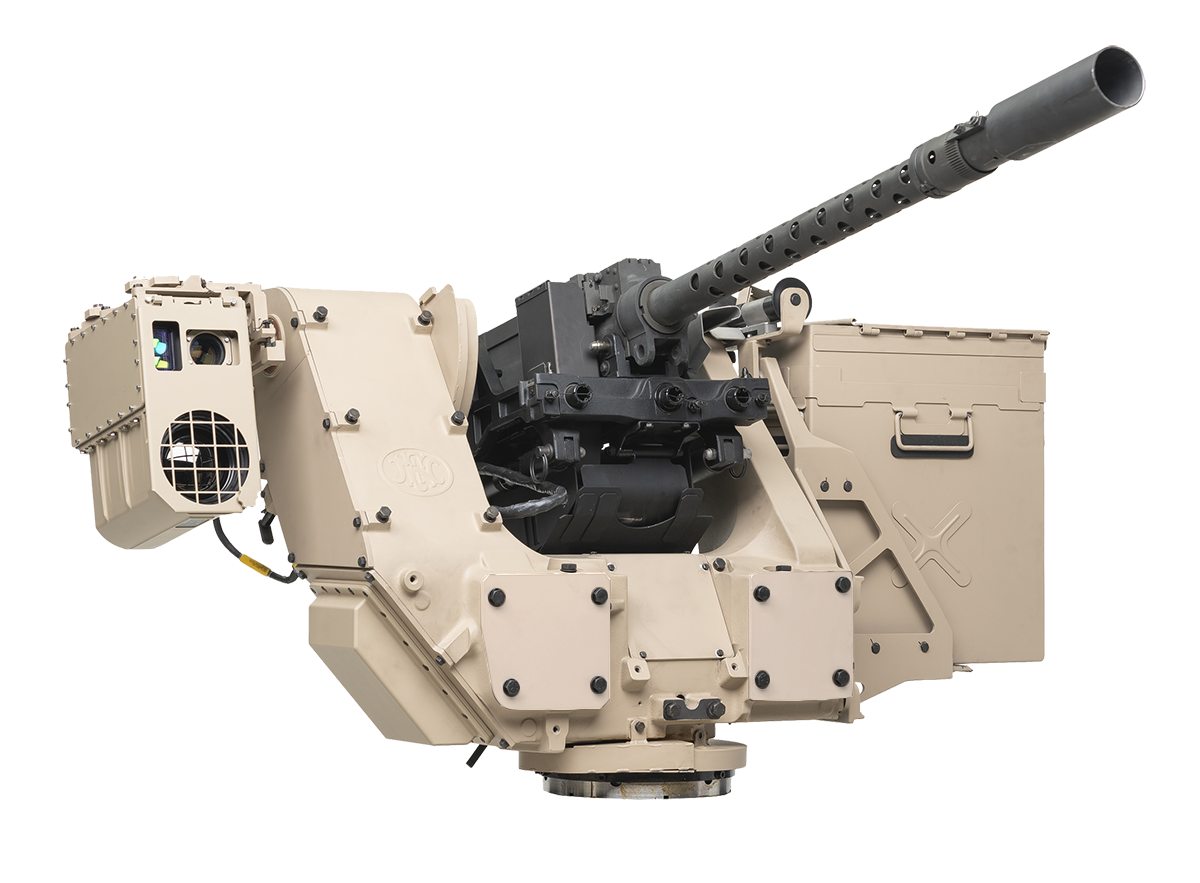
\includegraphics[width=.6\linewidth]{irod_defnder}
	\caption{A belga DeFNder rendszer \cite{defnder}}
	\label{fig:irod_defnder}
\end{figure}

Elég sok közös vonást találtam a fentebb említett rendszerekben. Az elrendezésük nagyon hasonló, van egy függőleges forgástengely nagyjából a teljes rendszer súlypontján keresztül, valamint egy vízszintes forgástengely, nagyjából a fegyver csövével egy síkban. Erre valószínűleg azért van szükség, hogy a tüzelés során keletkező erők ne ébresszenek csavarónyomatékot a mozgató mechanizmuson. Az én esetemben nagy erők nem fognak ébredni, de a tervezési elvet érdemes követni.

\paragraph{Samsung SGR-A1 \cite{samsung}}
Az egyetlen, valós harci helyzetben használt, teljesen autonóm gépágyú a koreai fejlesztésű \textsl{Samsung SGR-A1}. A két Korea között húzódó demilitarizált övezet (DMZ) egy 250 km hosszú, 4 km széles sáv, amelyet mind a két oldalon szigorúan ellenőriznek. A határ folyamatos felügyelete rengeteg ember munkájába kerül, ami egy demográfiai válságban lévő ország csökkenő hadseregében egyre értékesebb. Főleg annak tekintetében, hogy csupán járőrözni és figyelni a határt nem feltétlenül igényli egy ember jelenlétét. Ennek tudatában fejlesztették ki a Samsung és a Korea Egyetem mérnökei az SGR-A1 fegyverrendszert. Hőkamerával és éjjellátóval felszerelve napközben 4 km-ről, éjszaka 2 km-ről képes azonosítani potenciális célpontokat, tehát tulajdonképpen a DMZ teljes szélességében. Képes felismerni az embereket, követni őket, és megkülönböztetni az állatoktól. Hangfelismeréssel képes azonosítani a közeledő személyeket: amennyiben valaki 10 m-nél közelebb kerül és nem azonosítja magát, a rendszer riaszthat, gumilövedéket lőhet, vagy használhatja a K-3 gépfegyverét.

\begin{figure}[h!]
	\centering
	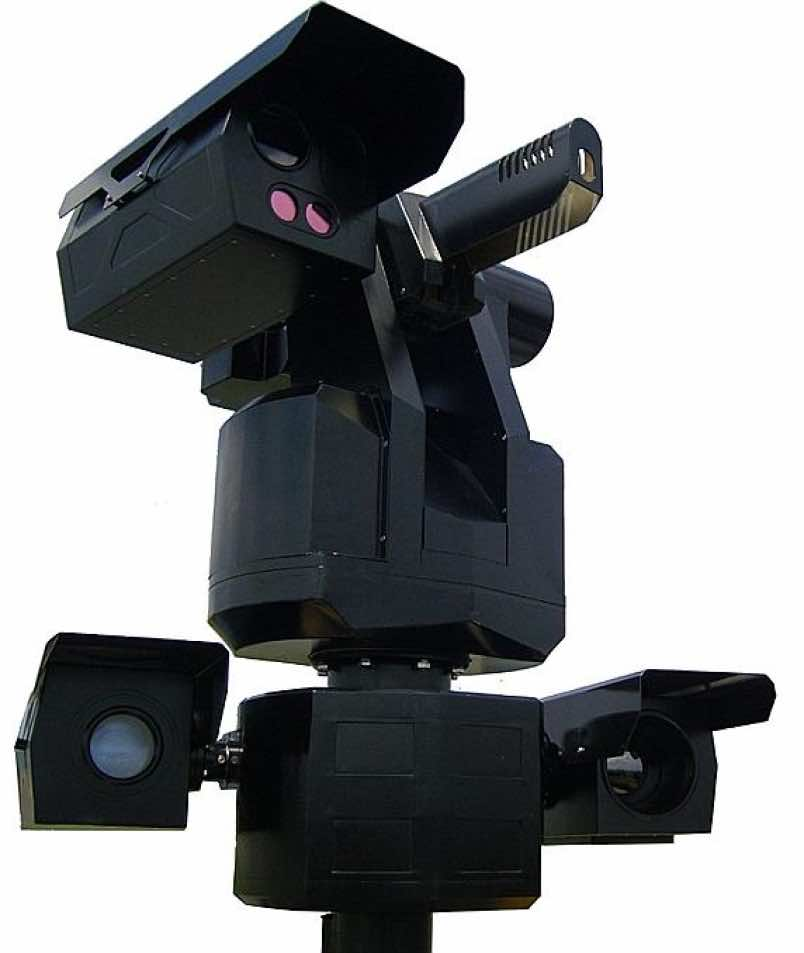
\includegraphics[width=0.35\linewidth]{irod_samsung}
	\caption{Samsung SGR-A1 \cite{samsung}}
	\label{fig:irod_samsung}
\end{figure}

Civil szakértők számára nem egyértelmű, hogy a rendszer lőhet-e emberi engedély nélkül, és a hivatalos koreai álláspont az, hogy nem. Azonban ha már bemérte és ellenségként azonosította a célpontot, akkor nehéz elképzelni, hogy pont a ravaszt ne tudná meghúzni.

\pagebreak

\section{Tüzelési mechanizmus}

A korábban említett rendszerek éles fegyverekkel vannak felszerelve, amit természetesen nem fogok követni. Így valamilyen olyan megoldást kellett találni, ami legális, elegendően pontos és megfelelően be lehet vele mutatni a célfelismerés és célzás működését. 


\paragraph{Paintball \cite{paintball}}

Több, a diplomamunkámhoz hasonló projektet is találtam, amelyek paintball puskákat használnak. Ezek a puskák sűrített levegőt alkalmaznak, hogy egy festékkel töltött golyót lőjenek ki. A torkolati sebességük nagyjából 280 fps, maximális hatékony távolságuk kb 25-30 m. Mivel a lövedék alakja gömb, és a cső sincs huzagolva, ezért nem túl pontos, főleg hosszú távon.\\

\begin{figure}[h!]
	\centering
	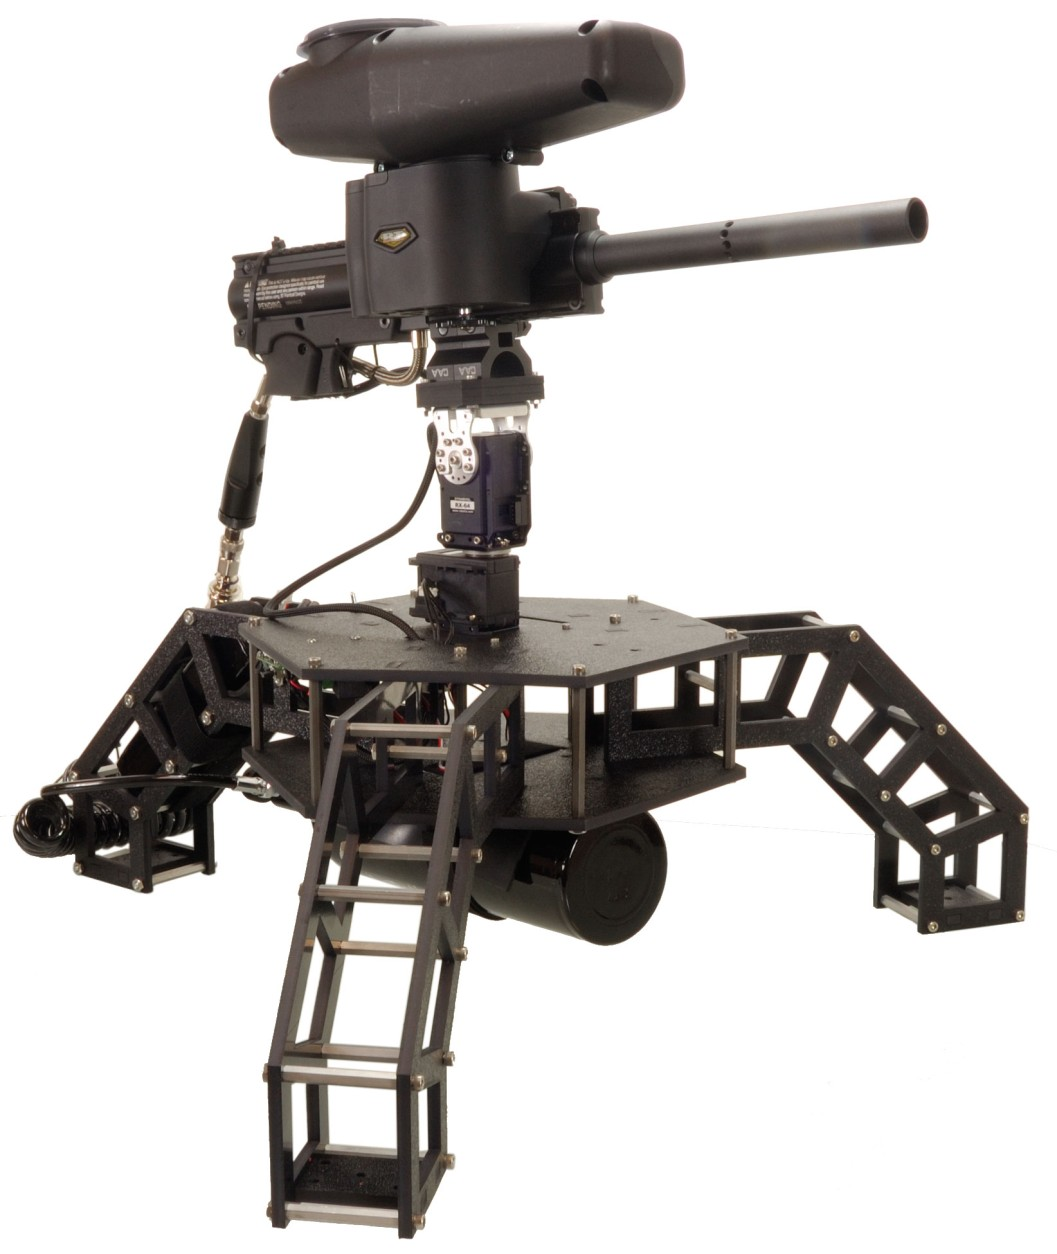
\includegraphics[width=0.4\linewidth]{irod_paintball}
	\caption{Paintball puska alapú rendszer \cite{paintballrobot}}
	\label{fig:irod_paintball}
\end{figure}

További problémák, hogy a legolcsóbb paintball puska is 70000 Ft. fölött van, valamint a lövedék is viszonylag drága, és nem lehet újrahasznosítani. Ezentúl a fegyverek nagyok, nehezek, és ezért nehéz a beépítésük. 


\paragraph{Nerf \cite{nerf}}

A Nerf fegyverek a legelterjedtebb játékfegyverek. Sűrített levegővel lőnek ki egy hosszúkás szivacs lövedéket. A sűrített levegőt egy megfeszített rugó elengedésével érik el, amelyet vagy kézzel, vagy valamilyen áttételes villanymotorral húznak fel. A legjobb modellek torkolati sebessége 70 fps körül van, és kb. 15 m a hatótávolságuk. Ezen a távon viszonylag pontosak a lövedék kialakításából adódóan, de jelentős az esés, így a ballisztikai pályát komolyan kell venni. \\

Ezek a fegyverek modelltől függően 10000 Ft. - 40000 Ft. között mozognak, de a lövedékeket újra lehet használni. Az a probléma itt is fennáll, hogy nagy a fegyver teste, így nehezebb beépíteni. 

\paragraph{Airsoft \cite{airsoft}}

Az airsoft fegyverek hasonló módon működnek, mint a Nerf puskák, de egy kisebb, műanyag golyót lőnek. Az elektromos airsoft fegyverek torkolati sebessége általában 300 fps és 400 fps között van, ami befolyásol a golyók tömege, a rugó minősége és rengeteg egyéb alkatrész. A hatótávjuk az átlagos fegyvereknek kb. 50 m, de fejlesztésekkel elérheti a 90 m-t is. A lövedék itt is golyó és a cső sincs huzagolva, mint a paintballnál, azonban az airsoft esetében használnak ún. hop-up kamrákat, amelyek perdületet adnak a golyónak.\\

Az airsoft fegyverek legnagyobb előnye a többi lehetőséggel szemben, hogy van egy kompakt egység, a "gearbox", ami felelős az elsütésért. Ezt ki lehet szedni egy fegyverből, vagy akár külön is meg lehet venni. Ez okkal nagyobb szabadságot ad a beépítéshez, és a végeredmény is sokkal kompaktabb lesz. Az elsütés is csak az áramkör zárását jelenti a gearboxban, ami egyszerűen vezérelhető a mikrokontrollerrel.